\section{Descrizione del prodotto}
\subsection{Obiettivi del prodotto}
L'obiettivo del prodotto è quello di sviluppare una piattaforma di monitoraggio per una città intelligente che consenta alle autorità locali di avere una visione d'insieme delle condizioni della città, permettendo loro di prendere decisioni informate e tempestive riguardo ad eventuali interventi e ottimizzazioni dei servizi da effettuare.

\subsection{Architettura del prodotto}
Il prodotto è costituito da 4 componenti principali.
	\subsubsection*{Simulatore} 
	Rappresenta la sorgente di dati. In uno scenario reale, i dati sono raccolti da migliaia di sensori installati nelle varie città. La \href{https://7last.github.io/docs/pb/documentazione-interna/glossario\#proponente}{proponente\textsubscript{G}} richiede che i dati siano i più realistici possibili, non escludendo la possibilità di inserire rilevazioni provenienti da sensori reali. Abbiamo scelto di utilizzare \href{https://7last.github.io/docs/pb/documentazione-interna/glossario\#python}{Python\textsubscript{G}} come linguaggio di programmazione per la simulazione dei dati in quanto è uno strumento molto flessibile che rende disponibili numerose librerie per la manipolazione dei dati.
	\subsubsection*{Piattaforma di streaming}
	Svolge la funzione di \href{https://7last.github.io/docs/pb/documentazione-interna/glossario\#broker}{broker\textsubscript{G}} per disaccoppiare lo stream di informazioni provenienti dai simulatori dei sensori. Si occupa di ricevere i dati provenienti dal simulatore e di inviarli ai vari consumatori. In questo caso, il consumatore principale è il database di cui al punto successivo. A tal fine, abbiamo deciso di utilizzare \href{https://7last.github.io/docs/pb/documentazione-interna/glossario\#Redpanda}{Redpanda\textsubscript{G}} come piattaforma di streaming, in quanto, sulla base dell'analisi eseguita, risulta avere prestazioni migliori rispetto ad \href{https://7last.github.io/docs/pb/documentazione-interna/glossario\#apache-kafka}{Apache Kafka\textsubscript{G}} mantenendo la compatibilità con le sue API.
	\subsubsection*{Database}
	Necessario per la persistenza dei dati raccolti. Per questo scopo abbiamo scelto di adottare \href{https://7last.github.io/docs/pb/documentazione-interna/glossario\#clickhouse}{ClickHouse\textsubscript{G}}, un database colonnare in grado di effettuare query analitiche complesse su grandi volumi di dati in modo molto efficiente.
	\subsubsection*{\href{https://7last.github.io/docs/pb/documentazione-interna/glossario\#dashboard}{Dashboard\textsubscript{G}}}
	Permette di visualizzare in tempo reale i dati raccolti. Questo componente rappresenta l'interfaccia utente del prodotto. Abbiamo scelto di utilizzare \href{https://7last.github.io/docs/pb/documentazione-interna/glossario\#grafana}{Grafana\textsubscript{G}} come strumento per la creazione di questa in quanto offre una vasta gamma di \href{https://7last.github.io/docs/pb/documentazione-interna/glossario\#dashboard}{dashboard\textsubscript{G}} interattive e dinamiche.


\begin{center}
	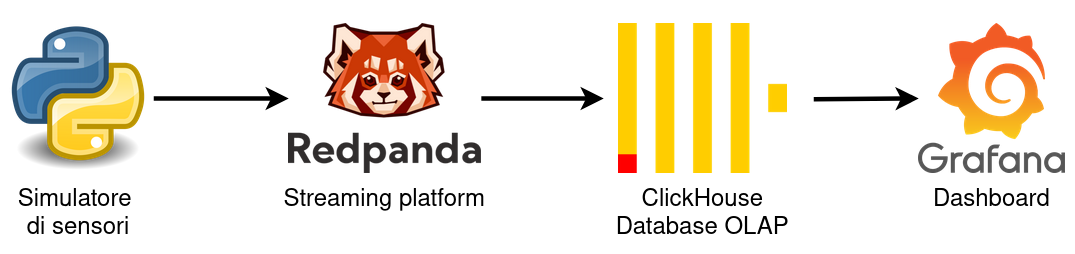
\includegraphics[width=0.8\textwidth]{analisi_dei_requisiti/stack}
	\captionof{figure}{Architettura del prodotto}
\end{center}

\subsection{Funzionalità del prodotto}
Una volta che il sistema sarà funzionante, esso potrà:
\begin{itemize}
	\item \textbf{raccogliere} e \textbf{memorizzare} i dati provenienti dalle diverse tipologie di sensori;
	\item \textbf{visualizzare} i dati raccolti in tempo reale attraverso una \href{https://7last.github.io/docs/pb/documentazione-interna/glossario\#dashboard}{\textbf{dashboard}\textsubscript{G}}, offrendo la possibilità di applicare filtri di diversa tipologia e fornendo una panoramica delle condizioni della città (tra le informazioni visualizzate ci saranno una mappa con la posizione dei sensori e alcuni grafici che mostrano gli andamenti delle misurazioni);
	\item \textbf{calcolare} un \textbf{Key Performance Index} (\href{https://7last.github.io/docs/pb/documentazione-interna/glossario\#key-performance-indicator}{KPI\textsubscript{G}}) della città, rappresentativo della qualità dei servizi forniti, basato sulle ultime rilevazioni dei sensori;
	\item \textbf{notificare} automaticamente le autorità locali in caso di superamento di soglie critiche da parte dei sensori.
\end{itemize}

\subsection{Caratteristiche degli utenti}
Si prevede che i principali utenti saranno le autorità locali \href{https://7last.github.io/docs/pb/documentazione-interna/glossario\#responsabile}{responsabili\textsubscript{G}} del monitoraggio dello stato di salute, sicurezza ed efficienza della città. Gli utenti interagiranno con il sistema esclusivamente attraverso la \href{https://7last.github.io/docs/pb/documentazione-interna/glossario\#dashboard}{dashboard\textsubscript{G}}.

\subsubsection{Conoscenze e competenze}
Si presume che tali utenti siano in grado di comprendere i dati visualizzati nella \href{https://7last.github.io/docs/pb/documentazione-interna/glossario\#dashboard}{dashboard\textsubscript{G}} e filtrare le informazioni per ottenere una visione d’insieme della situazione.

\subsubsection{Dispositivi}
Per accedere alla piattaforma gli utenti potranno utilizzare indifferentemente un dispositivo mobile, un computer o un tablet.